
% Lecture Template for ME3023 -  Measurements in Mechanical Systems - Tennessee Technological University
% Spring 2020 - Summer 2020 - Fall 2020 - Spring 2021 - Summer 2021
% Tristan Hill, May 07, 2020 - June 12, 2020 - July 08, 2020 - Novemeber 02, 2020 - March 28, 2021 - May 25, 2021
% Module Name: - Introduction
% Topic 2 - Types of Variables

\documentclass[fleqn]{beamer} % for presentation (has nav buttons at bottom)

%\usepackage{/home/thill/courses/measurements_lectures/measurements_lectures}
\usepackage{/home/tntech.edu/thill/courses/measurements_lectures/measurements_lectures}

\author{ME3023 - Measurements in Mechanical Systems} % original formatting from Mike Renfro, September 21, 2004

\newcommand{\TNUM}{2\hspace{2mm}} % Topic number 
\newcommand{\moduletitle}{Introduction}
\newcommand{\topictitle}{Types of Variables}

\newcommand{\sectiontitleI}{Measured Variable}
\newcommand{\sectiontitleII}{Independent and Dependent Variables}
\newcommand{\sectiontitleIII}{Controlled Variables and Parameters}
\newcommand{\sectiontitleIV}{Extraneous Variables}
\newcommand{\sectiontitleV}{Engineering Examples}

% custom box
\newsavebox{\mybox}

\title{Lecture Module - \moduletitle}

\date{Mechanical Engineering\vspc Tennessee Technological University}


\begin{document}

\lstset{language=MATLAB,basicstyle=\ttfamily\small,showstringspaces=false}

\frame{\titlepage \center\begin{framed}\Large \textbf{Topic \TNUM - \topictitle}\end{framed} \vspace{5mm}}

% Section 0: Outline
	\begin{frame}
		\large \textbf{Topic \TNUM - \topictitle} \vspace{3mm}\\
		\begin{itemize}

			\item \hyperlink{sectionI}{\sectiontitleI} \vspc % Section I
			\item \hyperlink{sectionII}{\sectiontitleII} \vspc % Section II
			\item \hyperlink{sectionIII}{\sectiontitleIII} \vspc %Section III
			\item \hyperlink{sectionIV}{\sectiontitleIV} \vspc %Section IV
			\item \hyperlink{sectionV}\sectiontitleV 	\vspc %Section IV

		\end{itemize}

	\end{frame}

% Section 1
\section{\sectiontitleI}
	\begin{frame}[label=sectionI]
		\frametitle{\sectiontitleI}

		\large{``A {\BL \hspcu} is an act of assigning a specific value to a physical variable. That physical variable
		is the {\GR measured variable}.''} \vspc
		{\tiny Text: Theory and Design of Mech. Meas.}

	\end{frame}

% Section 2
\section{\sectiontitleII}
	\begin{frame}[label=sectionII]
		\frametitle{Independent and Dependent Variables}

		{``If a change in one variable will not affect the value of some other variable, the
		two are considered independent of each other. A variable that can be changed independently of other
		variables is known as an {\PR \hspcu\hspc\hspcu}. A variable that is affected by changes in one or more
		other variables is known as a {\BR \hspcu\hspc\hspcu}. Normally, the variable that we measure depends on
		the value of the variables that control the process.''} \vspc
		{\tiny Text: Theory and Design of Mech. Meas.}

	\end{frame}

% Section 3
\section{\sectiontitleIII}
	\begin{frame}[label=sectionIII]
		\frametitle{\sectiontitleIII}

		{``A variable is {\BL \hspcu} if it can be held at a constant value
		or at some prescribed condition during a measurement... ...complete control of a variable is not usually
		possible. We use the adjective {\BL \hspcu} to refer to a variable that can be held as prescribed, at
		least in a nominal sense... \vspc
		...we define a {\GR \hspcu} as a functional grouping of variables. For example, a moment of inertia or a Reynolds number... ...A {\GR \hspcu} that has an effect on the behavior of the measured variable is called a control \hspcu....''} \vspc
		{\tiny Text: Theory and Design of Mech. Meas.}

	\end{frame}

% Section 4
\section{\sectiontitleIV}
	\begin{frame}[label=sectionIV]
		\frametitle{\sectiontitleIV}

		{``Variables that are not or cannot be controlled during measurement but that affect the value of the
		variable measured are called {\RD \hspcu\hspc\hspcu}. Their influence can confuse the clear relation
		between cause and effect in a measurement... ...The effects due to {\RD \hspcu\hspc\hspcu} can take the form of signals superimposed
		onto the measured signal with such forms as {\PR \hspcu} and drift.''} \vspc
		{\tiny Text: Theory and Design of Mech. Meas.}

	\end{frame}

% Section 5
\section{\sectiontitleV}
	\begin{frame}[label=sectionV]
		\frametitle{\sectiontitleV}
			\tiny
		
	        \begin{multicols}{2}
		
		    \textbf{Example 1: SHARP IR Ranger } \vspc
		    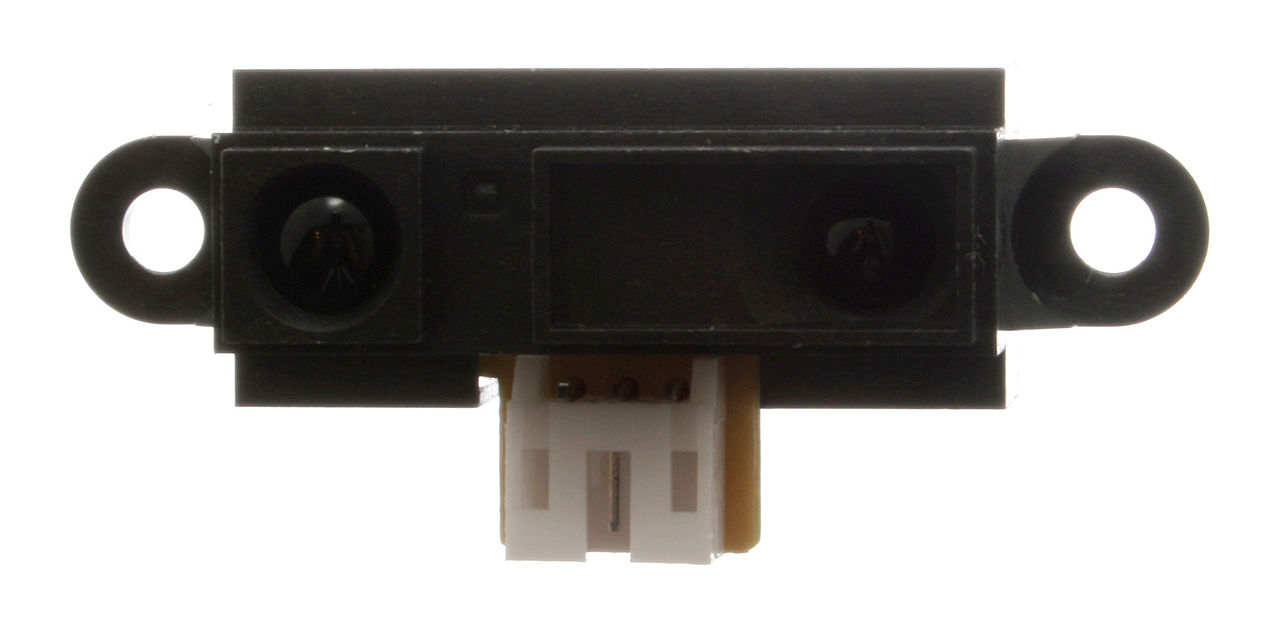
\includegraphics[scale=0.5]{proximity_sensor.jpg}
		    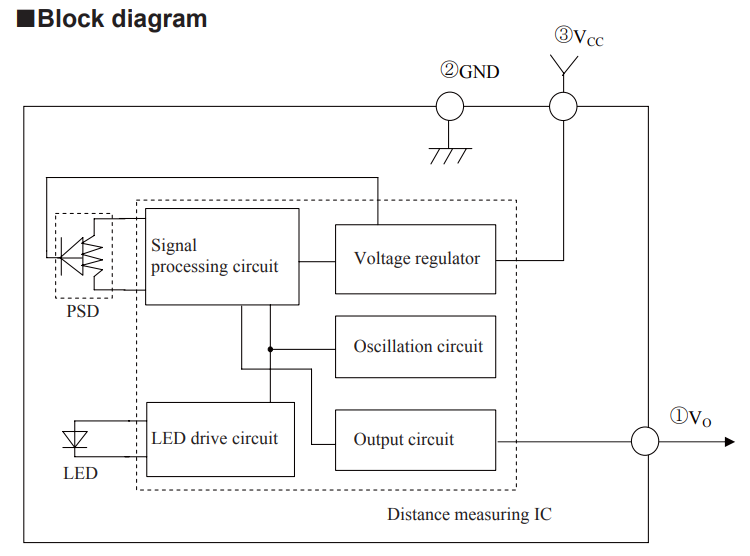
\includegraphics[scale=0.15]{sharp_ranger_circuit.png} \vspccc

		    Identify the following measurement stages 
		    \begin{itemize}
		    	\item Sensor: \hspcu
		    	\item Transducer: \hspcu
		    	\item Signal Conditioning: \hspcu
		    	\item Output: \hspcu
		    \end{itemize}


		    Name at least one for each of the following categories 
	
			\begin{itemize}
				\item Measured Variable: \hspcu \vspc 
				\item Independent Variable(s): \hspcu \vspc
				\item Dependent Variable(s): \hspcu, \hspcu \vspc 
				\item Controlled Variable(s): \hspcu, \hspcu \vspc 
				\item Extraneous Variable(s):\hspcu \vspc
			\end{itemize}
			
			\end{multicols}	

			{\tiny Image, More Info: \href{https://en.wikipedia.org/wiki/Proximity_sensor}{Wikipedia} }\hspace{40mm} {\tiny Image, More Info: \href{https://en.wikipedia.org/wiki/Position_sensitive_device}{Wikipedia} }

	\end{frame}

	\begin{frame}[label=sectionV]
		\frametitle{\sectiontitleV}
			\tiny
		
	        \begin{multicols}{2}
		
		    \textbf{Example 2: Thermocouple with DMM} \vspc
		    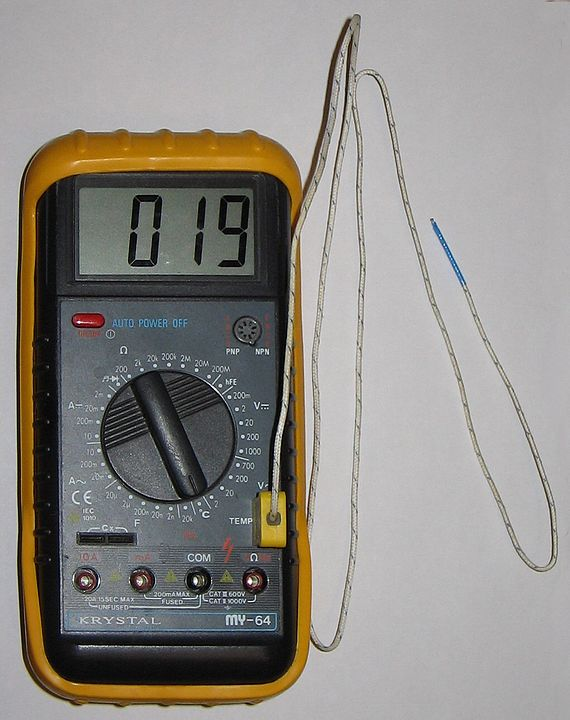
\includegraphics[scale=0.35]{thermocouple.jpg}
		    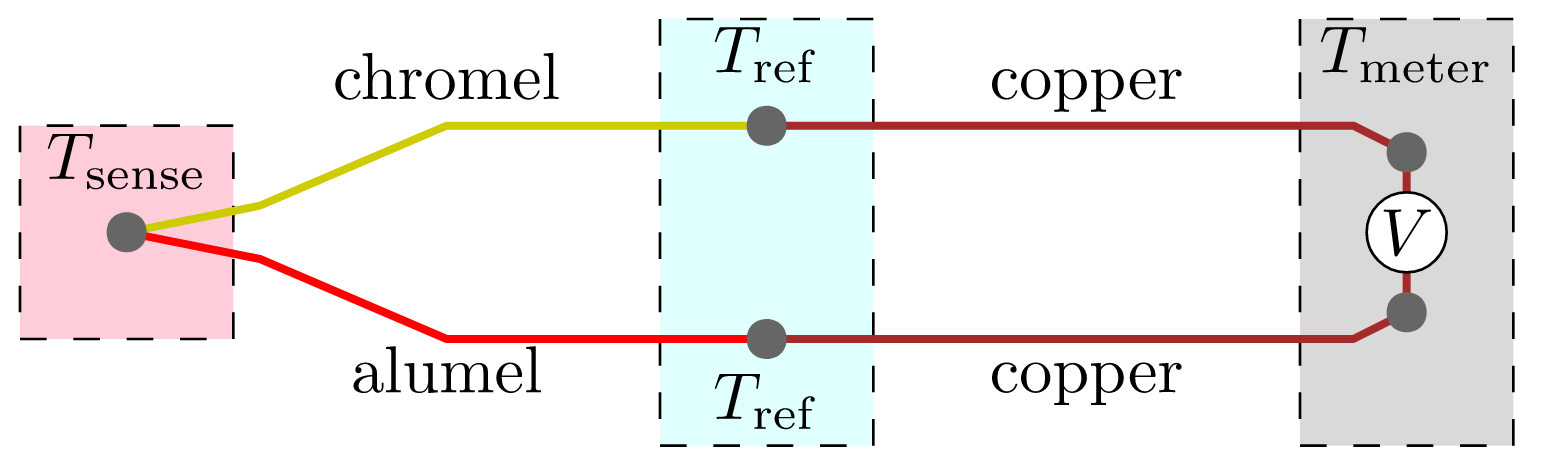
\includegraphics[scale=0.1]{thermocouple_concept.png} \vspc

		    Identify the following measurement stages 
		    \begin{itemize}
		    	\item Sensor: \hspcu
		    	\item Transducer: \hspcu
		    	\item Signal Conditioning: \hspcu
		    	\item Output: \hspcu
		    \end{itemize}


		    Name at least one for each category 
	
			\begin{itemize}
				\item Measured Variable: \hspcu \vspc 
				\item Independent Variable(s): \hspcu, \hspcu \vspc
				\item Dependent Variable(s): \hspcu, \hspcu \vspc 
				\item Controlled Variable(s): \hspcu \vspc 
				\item Extraneous Variable(s):\hspcu \vspc
			\end{itemize}
			
			\end{multicols}	

			{\tiny Image, More Info: \href{https://en.wikipedia.org/wiki/Thermocouple}{Wikipedia} }\hspace{40mm} 

	\end{frame}
\end{document}





